%% CAIN 2027 -- Research Track, SHORT research paper
%% Limit: 5 pages plus a maximum of 2 pages containing ONLY references.
%% Format: IEEE conference proceedings template; title 24pt, text 10pt;
%%        LaTeX must use \documentclass[10pt,conference]{IEEEtran}.
%% Double-anonymous review.
\documentclass[10pt,conference]{IEEEtran}
\IEEEoverridecommandlockouts

\usepackage{cite}
\usepackage{amsmath,amssymb}
\usepackage{booktabs}
\usepackage{xcolor}
\usepackage{tikz}
\usetikzlibrary{arrows.meta,positioning,patterns}
\usepackage[hidelinks]{hyperref}

\newcommand{\killk}[1]{Kill@#1}
\definecolor{oaccent}{HTML}{2F5D8C}
\definecolor{ofail}{HTML}{A5372F}
\definecolor{opass}{HTML}{2C6B4D}
\definecolor{orule}{HTML}{B9C2CE}

\begin{document}

\title{Evaluation Integrity as an Engineering Concern:\\
Receipts, Split Isolation and Rehearsal for\\
AI-Enabled Testing Systems}

\author{\IEEEauthorblockN{}\IEEEauthorblockA{}}

\maketitle

\begin{abstract}
An AI-enabled testing system is only as trustworthy as the machinery that
measures it, and that machinery is software with its own defects. We report the
engineering of an evaluation harness for an LLM-based mutation test generator,
and what it cost when one control was missing. Frozen hash-bound receipts,
structural split isolation and retained raw outputs let us establish that a
$9.04$ point gain on a checkpoint-selection panel corresponded to $+3.4346$
points on a locked split at exact McNemar $p = 0.0783$, failing a predeclared
$p < 0.01$ and retaining the untrained base model --- and that candidate
reference validity regressed $11.8726$ points over the same comparison while
parse and execution validity did not. One control was absent: no stage of the
one-time final measurement path had ever been executed against real data. That
measurement was authorized and consumed without producing anything, because a
record-admission rule ran before the scope filter that the production evaluator
applied first. We introduce a receipt-bound, full-scale rehearsal on a permitted
split as a standing pre-measurement gate; it reproduced a previously recorded
value exactly, establishing execution fidelity without touching the consumed
split. We argue that such gates are an AI-engineering deliverable, not
incidental tooling.
\end{abstract}

\begin{IEEEkeywords}
AI engineering, evaluation integrity, MLOps, provenance, software testing,
quality assurance
\end{IEEEkeywords}

\section{Introduction}

Systems with learned components are evaluated by systems without them, and the
second kind is ordinary software: it has defects, it drifts, and it is rarely
tested as carefully as the model it judges. The AI-engineering literature has
documented the operational burden of ML systems
\cite{sculley2015debt,amershi2019seforml} and the reproducibility problems that
follow \cite{gundersen2018reproducibility,pineau2021reproducibility}; leakage is
a recognised cause of overstated results \cite{kapoor2023leakage}. Less
attention is paid to the harness as a build artifact with its own quality
requirements.

This short paper reports that engineering problem concretely. It is not a paper
about a new model. The model here is a small open-weights code LLM used
unchanged, and the contribution is the measurement infrastructure around it:
what it caught, what it failed to catch, and what the failure cost.

\section{The System and Its Controls}

The system generates unit tests intended to distinguish a mutated function from
its correct implementation, scored by \killk{k} --- the fraction of targets for
which one of the first $k$ candidates kills the mutant. Fig.~\ref{fig:arch}
shows the evaluation architecture and where each integrity control sits.

\begin{figure*}[t]
\centering
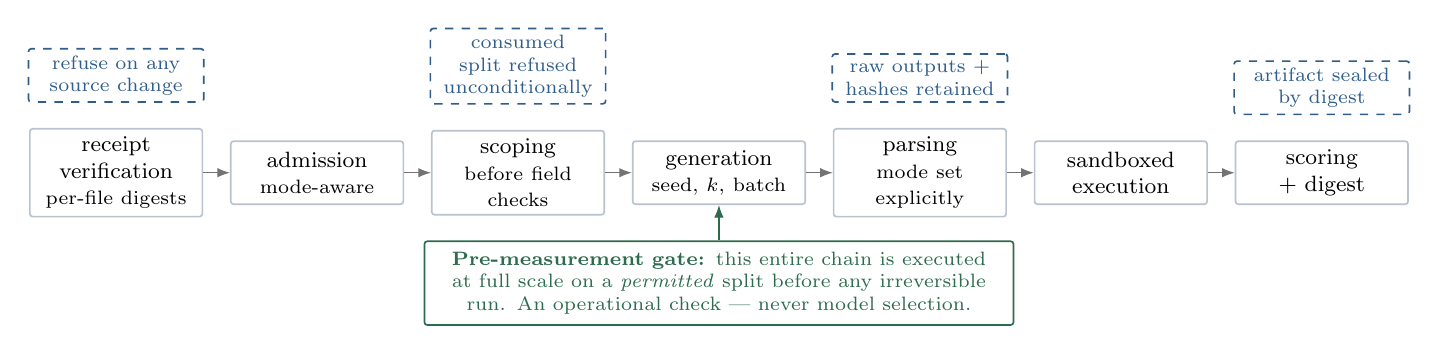
\begin{tikzpicture}[
  font=\footnotesize,
  st/.style={draw=orule,line width=0.6pt,rounded corners=1pt,
             text width=1.98cm,align=center,inner sep=3pt,minimum height=0.8cm},
  ct/.style={draw=oaccent,line width=0.6pt,rounded corners=1pt,dashed,
             text width=2.05cm,align=center,inner sep=2.5pt,font=\scriptsize,
             text=oaccent},
  a/.style={-{Latex[length=1.6mm]},draw=black!55}
]
\node[st] (rcpt) {receipt verification\\\scriptsize per-file digests};
\node[st,right=3.4mm of rcpt] (adm) {admission\\\scriptsize mode-aware};
\node[st,right=3.4mm of adm] (scope) {scoping\\\scriptsize before field checks};
\node[st,right=3.4mm of scope] (gen) {generation\\\scriptsize seed, $k$, batch};
\node[st,right=3.4mm of gen] (parse) {parsing\\\scriptsize mode set explicitly};
\node[st,right=3.4mm of parse] (exec) {sandboxed execution};
\node[st,right=3.4mm of exec] (score) {scoring + digest};

\node[ct,above=3.2mm of rcpt] {refuse on any source change};
\node[ct,above=3.2mm of scope] {consumed split refused unconditionally};
\node[ct,above=3.2mm of parse] {raw outputs + hashes retained};
\node[ct,above=3.2mm of score] {artifact sealed by digest};

\foreach \a/\b in {rcpt/adm, adm/scope, scope/gen, gen/parse, parse/exec, exec/score}
  {\draw[a] (\a) -- (\b);}

\node[draw=opass,line width=0.6pt,rounded corners=1pt,below=4.5mm of gen,
      text width=7.2cm,align=center,inner sep=4pt,text=opass,font=\scriptsize]
  (reh) {\textbf{Pre-measurement gate:} this entire chain is executed at full
  scale on a \emph{permitted} split before any irreversible run.
  An operational check --- never model selection.};
\draw[a,draw=opass] (reh.north) -- (gen.south);
\end{tikzpicture}
\caption{Evaluation architecture for an AI-enabled testing system. Dashed boxes
are integrity controls. The green gate is the control this project lacked, and
added only after losing a one-time measurement.}
\label{fig:arch}
\end{figure*}

Four controls were in place from the start.
\textbf{Frozen receipts}: the generation protocol, the evaluation scope and the
decision rule are committed to hash-bound JSON artifacts before the run they
govern, and every source file that can change a result is bound by an individual
digest rather than a whole-tree hash.
\textbf{Split isolation}: training, checkpoint-selection, locked and final
splits have distinct roles enforced in code.
\textbf{Raw-output retention}: every candidate retains its model output and a
digest of it.
\textbf{Explicit generation semantics}: parse mode, seed, batch size and
candidate count are recorded in the receipt and re-verified at run time.

\section{What the Controls Bought}

\begin{table}[t]
\caption{Headline measurement. The panels are not comparable quantities.}
\label{tab:main}
\centering
\footnotesize
\begin{tabular}{@{}llrr@{}}
\toprule
Panel & Arm & \killk{8} & Functions \\
\midrule
Development (selection-only, $n{=}542$) & base  & 0.605166 & 328 \\
                                        & A@431 & 0.695572 & 377 \\
\midrule
Locked ($n{=}757$) & base  & 0.594452 & 450 \\
                   & A@431 & 0.628798 & 476 \\
\midrule
\multicolumn{4}{@{}l}{\textit{Paired locked difference:} $+3.4346$ points,
$+114/-88$, net $+26$,} \\
\multicolumn{4}{@{}l}{exact McNemar $p = 0.0783$ vs.\ predeclared $p < 0.01$
--- \textbf{not met}.} \\
\multicolumn{4}{@{}l}{\textit{Decision:} retain the untrained base model.} \\
\multicolumn{4}{@{}l}{\textit{Reference validity:} $0.452114 \to 0.333388$
($-11.8726$ points), while} \\
\multicolumn{4}{@{}l}{parse ($+0.1486$) and execution ($+1.3870$) validity did
not regress.} \\
\bottomrule
\end{tabular}
\end{table}

Table~\ref{tab:main} summarises what the controls made reportable. Because the
decision rule was frozen in a hashed artifact before either locked arm ran, a
$p$ of $0.0783$ against a required $p < 0.01$ could not be renegotiated
afterwards, and the retention decision is interpretable. Because reference
validity was measured alongside \killk{k}, a substantial regression became
visible that a kill-rate-only harness would have missed --- and because parse
and execution validity were measured too, that regression could be isolated
rather than attributed to general degradation.

We state the evidential status precisely. The locked point estimate is
positive; the predeclared threshold was not met; that is insufficient evidence
of an effect, \textbf{not} evidence of no effect
\cite{wasserstein2016asa,amrhein2019retire}. Development figures are selection
statistics, since that panel chose the checkpoints it scored. No final-test
result exists, no repository-level kill rate exists, and no comparison against
any external baseline tool was run.

\section{The Control That Was Missing}

A fourth split was reserved for a single final measurement, protected by a
one-time authorization and a hash-bound receipt. It was authorized, attempted,
and consumed without producing a measurement: the authorization was spent and
the run raised while admitting records, yielding \textbf{zero candidates and
zero reportable metrics}. The split may never be rerun.

The cause is instructive because it is a pure engineering defect. The final-run
path required a fixed set of record fields to be non-empty on \emph{every}
record in the split, raising before returning any of them. Records of one
execution mode legitimately carry some of those fields blank, and the production
evaluator had always loaded the split and \emph{then} scoped scoring by mode.
The final path inverted that order.

Two properties made this expensive rather than merely annoying:

\begin{enumerate}
  \item \textbf{The component was designed to be unreachable} until the
        authorization was spent, so it had never been executed against real
        data. Six successive audits of the readiness receipt each found a real
        defect --- and every one of those defects was in something
        \emph{recorded} rather than \emph{executed}.
  \item \textbf{The guard asked the wrong question.} It gated on whether access
        had ever been authorized, a fact that once recorded never expires,
        rather than on whether anything remained to measure. A permission check
        is not an exhaustion check.
\end{enumerate}

\begin{table}[t]
\caption{Evaluation-integrity risks and the control each requires. Every
mitigation listed is implemented in the system described here.}
\label{tab:risk}
\centering
\scriptsize
\begin{tabular}{@{}p{0.30\columnwidth}p{0.60\columnwidth}@{}}
\toprule
\textbf{Risk} & \textbf{Implemented control} \\
\midrule
Decision rule adjusted after seeing results & Rule and thresholds committed to a
hash-bound receipt before the run; runtime refuses a receipt whose digest
differs \\
Silent change to code that defines a result & Per-file canonical digests for
every result-defining source; whole-tree hashes rejected as too noisy to act on \\
Same checkout appears to differ across platforms & Both a raw and a
line-ending-normalised digest recorded per file \\
Held-out split reached by ordinary code & Split roles enforced structurally;
consumed split refused unconditionally, with the read path deleted rather than
made unreachable \\
Score attributable to a scoring bug, unverifiable later & Raw model output plus
digest retained per candidate; digests independently recomputable \\
Measurement scored under the wrong parser & Parse mode written into the receipt
and set explicitly at run time, never inherited from a default \\
Quality regression hidden by the headline metric & Parse, execution and
reference validity reported alongside \killk{k} \\
Irreversible run executes never-run code & \textbf{Full-scale rehearsal on a
permitted split as a standing gate} \\
One failure consumes a one-time resource & Two-phase authorization: reserve on
open, commit only after the first batch scores \textit{(designed; not yet
implemented)} \\
\bottomrule
\end{tabular}
\end{table}

\section{The Rehearsal Gate}

The repair was not only to fix the admission rule but to remove the condition
that made it untestable. Admission now partitions by execution mode first and
applies field requirements only to records that will be scored, importing the
mode semantics from the production evaluator rather than restating them.

More importantly, we added the gate shown in Fig.~\ref{fig:arch}: before any
irreversible measurement, the entire chain executes at full scale on a permitted
split under a hash-bound receipt whose source bindings are verified before the
model loads. The first such rehearsal scoped $594$ requested records to $542$
scored targets with zero admission errors, generated $4{,}336$ candidates in
$271$ batches, retained $4{,}336$ raw outputs with $4{,}336$ digests, reported
zero missing and zero mismatched, and recorded zero mismatches on an independent
recomputation. It completed in $577.753$ seconds, wrote no weights and loaded no
adapter. Its \killk{8} was $0.605166$ --- identical to the value previously
recorded for the same model on the same panel under the same evaluation-scope
digest.

\textbf{That exact reproduction is a statement about code, not about the
model.} It establishes execution fidelity: the rebuilt path computes the same
number as the path that produced the historical value. It is not a
model-performance result, not a generalization estimate and not a selection
result. The rehearsal receipt carries
\texttt{final\_test\_measurement: false},
\texttt{eligible\_for\_model\_selection: false} and
\texttt{supports\_performance\_claim: false} as machine-checkable fields, and
the runner refuses any receipt lacking them --- an engineering choice that makes
the limitation enforceable rather than editorial.

\section{Why This Is an AI-Engineering Contribution}

Three reasons, stated plainly.

First, \textbf{the harness is the deliverable that determines whether any model
claim is admissible}. Our strongest empirical statements are negative or
inconclusive, and they are only reportable because the rule was frozen and the
provenance held. Infrastructure that makes a negative result publishable is
doing the same job as infrastructure that makes a positive one credible.

Second, \textbf{the defects we hit are software defects with software
remedies} --- ordering of a filter and a validator, a permission check standing
in for an exhaustion check, a component unreachable by design and therefore
untested. None required ML expertise to cause or to fix, and all of them
threatened the validity of an ML result.

Third, \textbf{irreversible evaluation resources need release engineering}. A
one-time held-out split is a resource that can be spent once and destroyed by a
crash in ordinary code. Treating it like a production deployment --- rehearse at
full scale, verify bindings before the expensive step, make the commit point
two-phase --- is the discipline the situation calls for, and it is ours to
supply.

\section{Threats to Validity}

One model, one corpus, one supervision family, one seed; we do not claim the
measured magnitudes transfer. \killk{k} credits any distinguishing candidate,
including a universally failing test, which is why reference validity is
reported beside it; mutants are an imperfect fault proxy
\cite{just2014mutants}. The locked comparison is a single paired exact test on
$202$ discordant pairs. One locked criterion failed through a defect of ours ---
an adapter-specific digest placed inside a contract required to be identical
across arms --- recorded as a failure rather than reinterpreted; the decision
does not rest on it. The two-phase authorization in Table~\ref{tab:risk} is
designed but not yet implemented, and is labelled as such.

\section{Conclusion}

Evaluation infrastructure for AI-enabled systems is software, and it fails in
software ways with scientific consequences. Frozen receipts, per-file source
binding, structural split isolation and retained raw outputs let us report a
locked result that did not meet its predeclared threshold, and a validity
regression that the headline metric concealed. Their absence in one place ---
a measurement path that had never been executed against real data --- consumed a
one-time resource and produced nothing. The gate that closes that hole is cheap
and repeatable: run the whole path, at full scale, on data you are allowed to
spend.

An anonymized replication package contains the frozen protocol, decision-rule
and result receipts, the rehearsal receipts, and per-figure data files carrying
their source digests. No material from the consumed split is included, and none
exists.

\bibliographystyle{IEEEtran}
\bibliography{references}

\end{document}
